\documentclass[12pt]{article}
\usepackage{epsfig}
\textwidth 7.5in                     % page width in inches
\textheight 9.9in                    % page height in inches
\topmargin -90pt                     % to fit on A4
\oddsidemargin -36pt                 % Left hand margin (odd pages)
\evensidemargin -28pt
\baselineskip 0.168in
\setlength{\parindent}{20pt}
%\def\etal{{\it et al. }}
\def\etal{et al.\ }
\newcommand{\msun}{\hbox{M$_{\odot}$}}

\begin{document}

\noindent
\centerline{\bf \textit{Shane Observations with UCSC ASTR 257: Modern Astronomical Techniques}} 
\centerline{\bf PI A.\ Skemer}

\vskip 15pt

\centerline{\bf  Scientific Justification: }

As part of UC Santa Cruz Astronomy's new graduate curriculum, I am developing a new observing class, which consists of a week-long field trip to Lick Observatory.  The class is required of all first-year graduate students, and ensures that (1) our students will develop a broad range of observational skills at a time when opportunities to develop these skills are becoming more rare, and (2) our students will develop experience with Lick Observatory facilities, which will incentives them to become immediate scientific users.  This class has some parallels to the graduate observing workshop that has been run for many years at Lick Observatory, but the formal course will be more time intensive and will fulfill specific department requirements.

We are planning two observations with the Shane 3-meter.  We will observe edge-on galaxies with the KAST spectrograph to replicate the Vera Rubin experiment, and we will observe Neptune with Shane-AO to make a 3-color image.  The edge-on galaxy experiment is a mainstay of the PHYS/ASTR 136 undergraduate course.  The Neptune image is a common AO demonstration observation.  We request 3 hours of KAST time for the galaxies observation and 2 hours of AO time for Neptune.  For scheduling reasons, we prefer these observations to take place at the beginning of the night.

\newpage


\begin{figure*}[t!]
  \centering
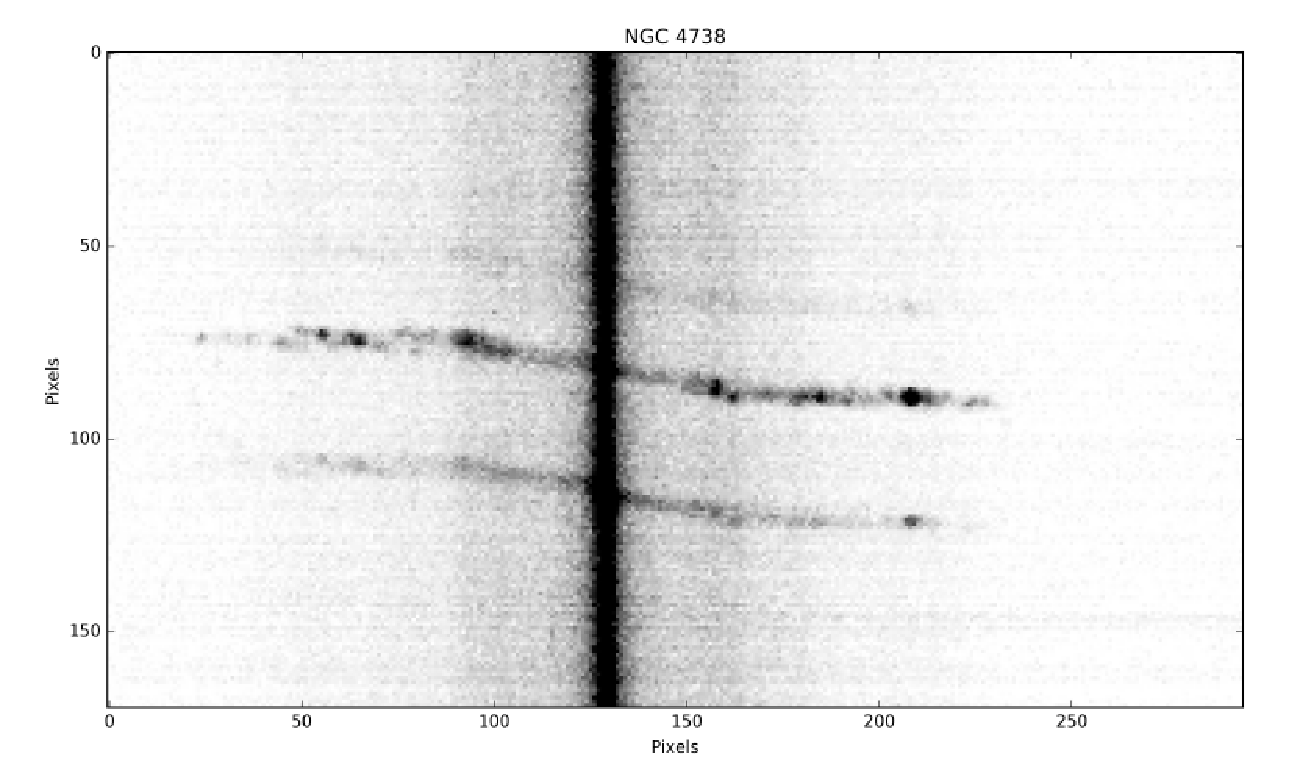
\includegraphics[width=15cm]{fig1.pdf}
  \caption{KAST dispersed image of an edge-on galaxy showing a flat rotation curve.  Image by PHYS 136 student, Zafar Rustamkulov.}
\end{figure*}

\begin{figure*}[t!]
  \centering
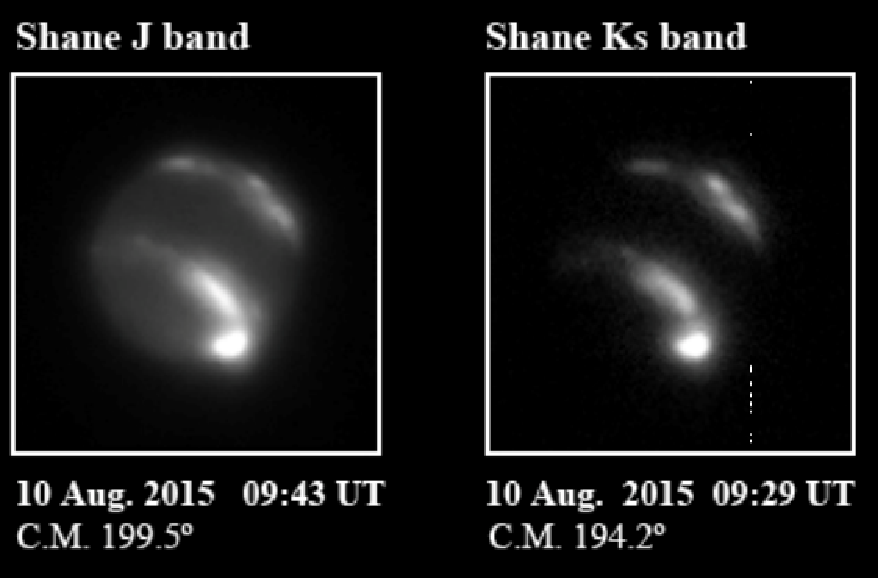
\includegraphics[width=15cm]{fig2.pdf}
  \caption{Shane-AO NGS image of Neptune at multiple wavelengths (Hueso et al. \textit{Icarus}, 2017).}
\end{figure*}

\clearpage

\newpage

\centerline{\bf Technical Remarks}

\noindent
{\bf Targets and Exposures}

\begin{table}[!h]
\begin{tabular}{lllllllllllll}
\hline
Name & instrument \\
\hline
NGC 4738-like objects             & KAST\\
Neptune             & Shane-AO NGS and SHARCS  \\
\hline
\end{tabular}
\end{table}
\noindent
{\bf Supplementary Observations}
None
\\\\
\noindent
{\bf Technical Remarks}
These observations have all been done before with Shane.
\\\\
\noindent
{\bf Path to Science from Observations}
N/A
\\\\
\noindent
{\bf Status of Previous 3-m Programs}
N/A

\end{document}